\section{CERN and the Large Hadron Collider}
The organisation européenne pour la recherche nucléaire or CERN is the organization that conducting the world's frontier particle physics experiments. It's a coalition of scientists representing numerous countries around the world, who work together for a greater understanding of the universe. CERN hosts the Large Hadron Collider, currently the largest particle collider in the world. It is 27 km in circumference and hosts eight experimental caverns 150 meters underneath the earth ~\cite{}. Accelerator physicists and engineers strive to provide high energy collisions along these eight sites. Monumental effort is made to guide the beam, utilizing more than 2000 superconducting magnets to steer, press, and shape the accelerating protons. Crossing points facilitated by crab-like magnets force these particles to cross, collide, and interact at the caverns where the experiments take data. Multiple campaigns for particle physics are done such as low intensity fills, lead-lead collisions, and proton collision. The Compact Muon Solenoid (CMS) is the general purpose proton-proton detector, located at P5 in Cessy, France, that took the data that will be analyzed in this dissertation. 

\begin{figure}[ht!b]
  \centering
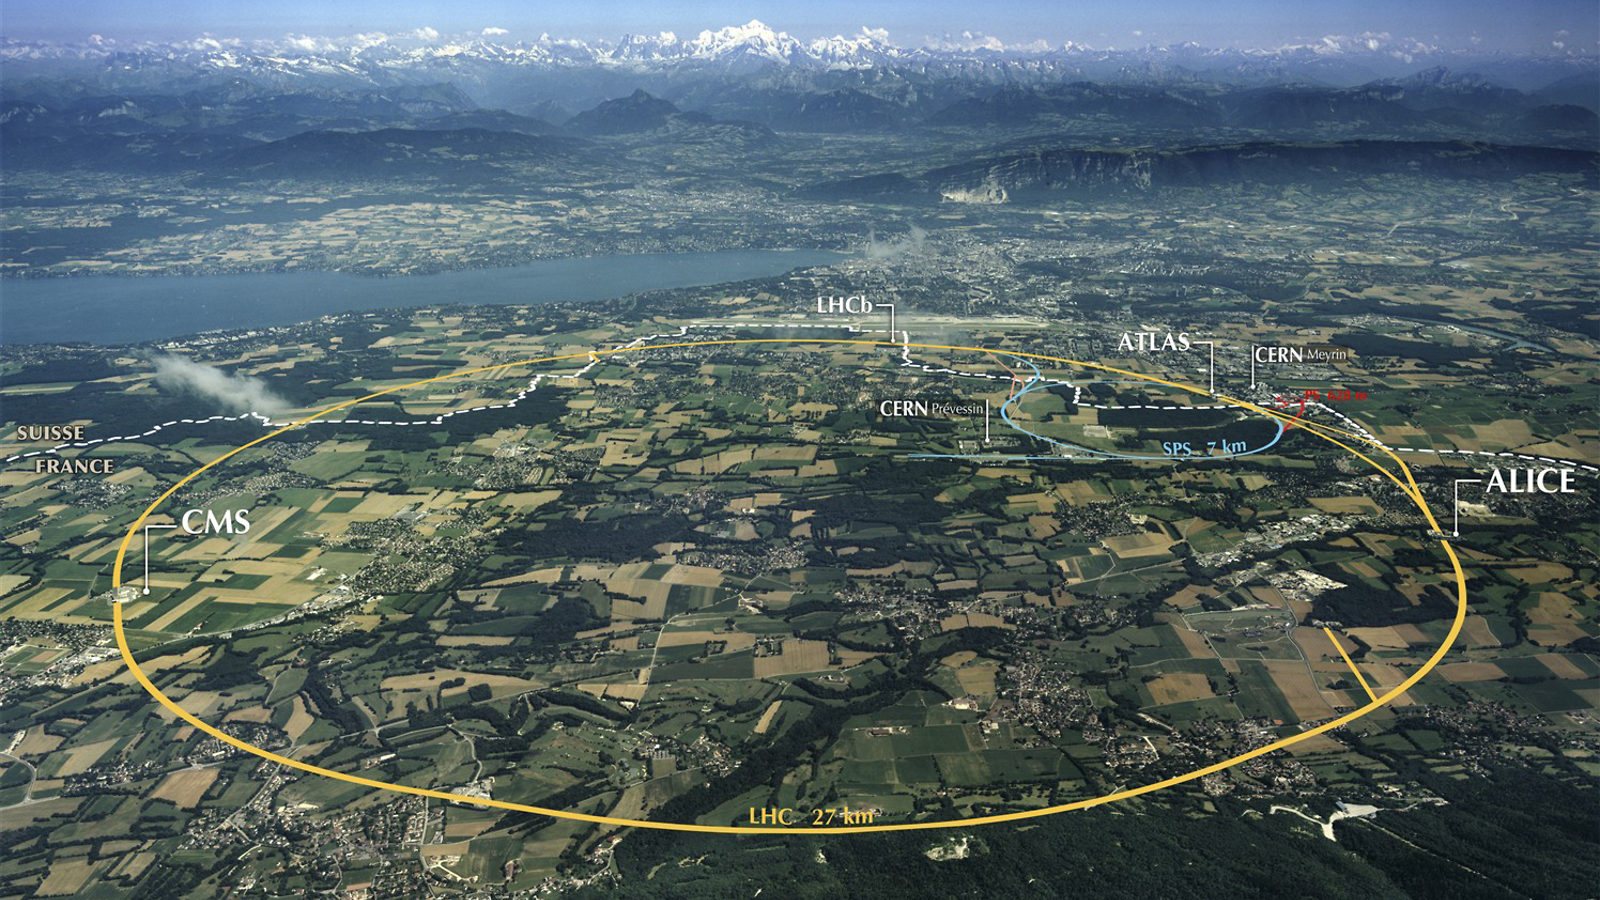
\includegraphics[width=0.75\textwidth]{figures/LHC_map-s.jpg}    
    \caption{\label{fig:lhc} Overview of the Large Hadron Collider spanning Switzerland and France - Maximilien Brice, CERN }
\end{figure}

\section{The Compact Muon Solenoid detector}
At 14,000 tonnes the CMS detector may not seem like it would be compact; however, it is quite dense. As shown in the diagram, the detector contains many sub-detector systems and also features the most powerful solenoid magnet ever made for it's size. At 6 meters inner diameter, and a combined weight of the solenoid and the steel return yolk of 12,500 tonnes it is the central feature of the Compact Muon Solenoid (CMS) \ref{fig:cmsdet}.
\begin{figure}[!htb]
\begin{center}
\includegraphics[width=0.75\textwidth]{Figures/cmsDet.png}
\label{fig:cmsdet}
\end{center}
\end{figure}
 Within the solenoid volume, there is the
silicon pixel and strip tracker, a lead tungstate crystal 
electromagnetic calorimeter (ECAL), and a brass and scintillator 
hadron calorimeter (HCAL), each composed of a barrel and two endcap 
sections. Forward calorimeters extend the pseudorapidity 
coverage provided by the barrel and endcap detectors. 
Muons are detected in gas-ionization chambers embedded 
in the steel flux-return yoke outside the solenoid.

From the central interaction point, the CMS detector hosts
the silicon pixel and strip tracker, the lead tungstate crystal electromagnetic
calorimeter (ECAL), and the brass-scintillator hadron calorimeter (HCAL),
each composed of a barrel and two endcap sections. The central feature of
the CMS apparatus is a superconducting solenoid of 6\unit{m} internal diameter, providing
a magnetic field of 3.8\unit{T}. The silicon pixel and tracking systems as well as
the calorimeters are contained within the solenoid volume.  %cite

The nominal $\Pp\Pp$ bunch crossing rate at the LHC is 40\unit{MHz}. This rate would be too extreme for any data taking system. In order to reduce the rate of events that are recorded for offline analysis, events of interest are selected using a two-step trigger system~\cite{Khachatryan:2016bia}.
The first level (L1) is composed of custom built electronics which makes use of
high speed optical links and large Field Programmable Gate Arrays (FPGAs). 
L1 reduces the event rate from the nominal bunch crossing to a rate of around
100\unit{kHz} within a time interval of less than 3.5\mus.
The second level, known as the High Level Trigger (HLT), consists of a farm of 
generic processors running a version of the full event reconstruction software that
 has been optimized for fast processing. The HLT reduces the event rate to about
1\unit{kHz} before data storage.

Since the 2012 data taking, significant upgrades of the L1 trigger 
have benefited this analysis, especially in the final state with two semi-hadronically decaying 
$\Pgt$ leptons, denoted as $\tauh$.  
These upgrades improved the $\tauh$ identification at L1 by giving more flexibility 
to object isolation, allowing new techniques to suppress the contribution from 
additional $\Pp\Pp$ interactions per bunch
crossing, and to reconstruct the L1 $\tauh$ object in a fiducial region that matches 
more closely that of a true $\tauh$ decay.

A more detailed description of the CMS detector, 
together with a definition of the coordinate system used and 
the relevant kinematic variables, can be found in Ref. ~\cite{Chatrchyan:2008zzk}.


\section{Subdetector Systems}
\subsection{Muon Identification Systems}
While all subdector systems are important to physics at CMS due to the reconstruction, there are a couple detectors that contribute to the particles that are identified in pseudoscalar search. These are the tracker system, muon system, and the hadronic calorimeter. With two muons and two tau leptons in the final state, muon and tau identification are paramount to the search. 

In order to identify good muons, several subdetector systems work together in order to reconstruct muons. Looking at muons that come from the interaction vertex - prompt muons - the tracker plays an important role in indentifying charged particle tracks. 

As CMS implies in it's name, muons are certainly a focal point in particle detection. Muon reconstruction is possible for the whole kinematic range of the LHC. The tracker system works in tandem with the gas chambers to reconstruct muons, and the solenoid accentuates charge particle's momentum allowing for the most accurate mass resolution possible in a hadronic based physics detector. The gas chambers comprise of Drift Tubes which cover a pseudorapidity region ($|\eta|<1.2$) split into 4 stations in the flux return plates. 

In the higher $|\eta|$ regions, cathode strip chambers (CSCs) are used and preferred for their fas response time, fine segmentation, and radiation resistance ~\cite{Chatrchyan:1129810}. For a visual representation of a cross section of the muon system please refer to figure \ref{fig:muonsystem}. Notably, the track of the muon is bent inside the solenoid by the Lorentz force, but outside of that the muon isn't curved in the typical helical fashion. 

During reconstruction, the particle flow algorithm ~\cite{CMS-PAS-PFT-09-001} can identify tracker or global muons which are ultimately divided into four sub types depending on the $\chi^2$ of the track reconstruction and momentum of the candidate muon ~\cite{Kratschmer:1956760}


\begin{figure}[ht!b]
  \centering
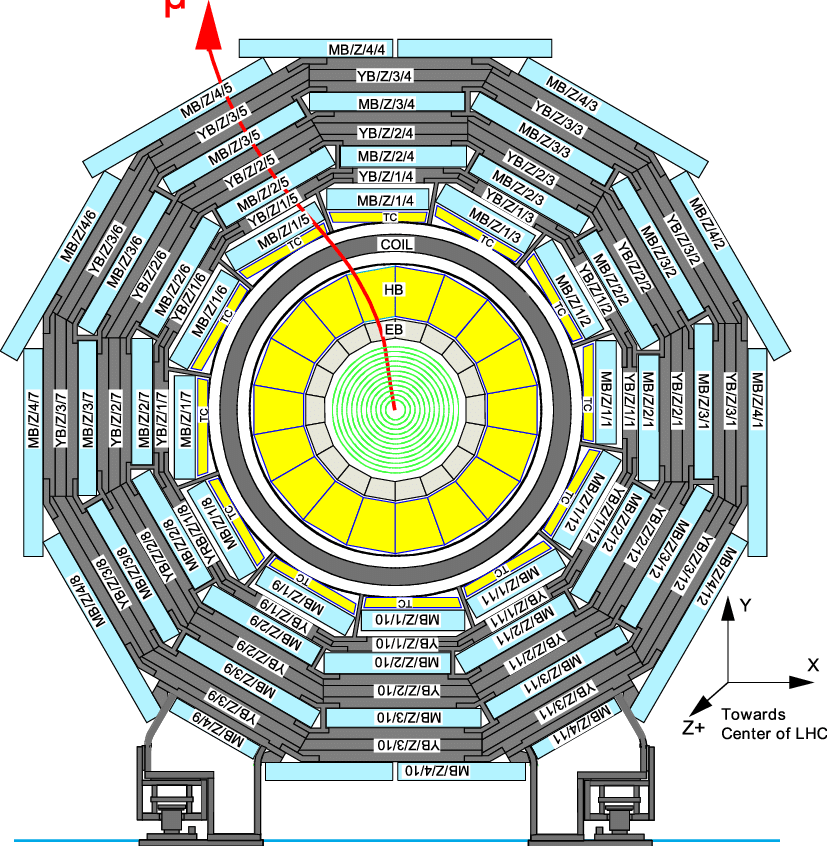
\includegraphics[width=0.75\textwidth]{figures/Layout-of-the-CMS-barrel-muon-DT-chambers-in-one-of-the-5-wheels-59.png}    
    \caption{\label{fig:muonsystem} Muon system involving multiple subtector systems: tracker, solenoid, and the muon gas chambers around the iron yoke (grey) - Maximilien Brice, CERN }
\end{figure}


\subsection{Tau Identification Systems}
Tau leptons are the probably the most interesting SM particle. They are leptons, that directly

physics of tau decay 
types of tau decay 
pions and intermediate mesons 
HPS

